\documentclass{ximera}
%herschreven 13/11/26
\title{Omzetten van eenheden}
\author{Daan Lipkens}

\begin{document}
\begin{abstract}
    Oppervlakte en volume, de liter, samengestelde eenheden en tijd omzetten.
\end{abstract}
\maketitle

\section{Oppervlakte en volume}\label{sec:omzetten_oppervlakte_volume}
Bij oppervlakte en volume staat de eenheid in het kwadraat of tot de derde macht. Die macht geldt ook voor de prefix: $1 \, \mathrm{cm}^{2}$ betekent $1 \, (\mathrm{cm})^{2}$.

\begin{proposition}[title={Omzetten van oppervlakte en volume}]\nl
    Vervang de prefix door zijn macht van 10 en verhef die macht mee in het kwadraat (oppervlakte) of tot de derde macht (volume):
    \[ 1 \, \mathrm{cm}^{2} = (10^{-2} \, \mathrm{m})^{2} = 10^{-4} \, \mathrm{m}^{2} \qquad\qquad 1 \, \mathrm{cm}^{3} = (10^{-2} \, \mathrm{m})^{3} = 10^{-6} \, \mathrm{m}^{3} \]
\end{proposition}

\begin{example}[foldable=true,title={Voorbeeld: vierkante centimeter naar vierkante meter}]\nl
    Een postzegel heeft een oppervlakte van $8{,}3 \, \mathrm{cm}^{2}$. Hoeveel vierkante meter is dit?

    \begin{solution}\nl
        \begin{align*}
            8{,}3 \, \mathrm{cm}^{2} &= 8{,}3 \cdot (10^{-2} \, \mathrm{m})^{2} && \text{(prefix c vervangen door $10^{-2}$)}\\
            &= \boxed{8{,}3 \cdot 10^{-4} \, \mathrm{m}^{2}} && \text{(macht kwadrateren)}
        \end{align*}
    \end{solution}
\end{example}

\begin{example}[foldable=true,title={Voorbeeld: kubieke meter naar kubieke micrometer}]\nl
    Hoeveel kubieke micrometer is $3{,}4 \, \mathrm{m}^{3}$?

    \begin{solution}\nl
        Van m ($10^{0}$) naar $\mu$m ($10^{-6}$) is een stap van $10^{0-(-6)} = 10^{6}$ voor de lengte. Voor een volume verhef je die stap tot de derde macht:
        \begin{align*}
            3{,}4 \, \mathrm{m}^{3} &= 3{,}4 \cdot (10^{6})^{3} \, \mathrm{\mu m}^{3} && \text{(stap tot de derde macht)}\\
            &= \boxed{3{,}4 \cdot 10^{18} \, \mathrm{\mu m}^{3}}
        \end{align*}
    \end{solution}
\end{example}

Voor vloeistoffen gebruik je vaak de liter als eenheid van volume.

\begin{definition}[title={Liter}]\nl
    De \textbf{liter} (symbool L) is een eenheid van volume:
    \[ 1 \, \mathrm{L} = 1 \, \mathrm{dm}^{3} = 10^{-3} \, \mathrm{m}^{3} \qquad \text{en dus} \qquad 1 \, \mathrm{mL} = 1 \, \mathrm{cm}^{3} \]
    Dit geldt voor elke stof, niet alleen voor water. Ook de kleine letter l is toegelaten, maar de hoofdletter L vermijdt verwarring met het cijfer 1.
\end{definition}

\begin{example}[foldable=true,title={Voorbeeld: centiliter naar kubieke meter en kubieke millimeter}]\nl
    Een fles bevat $75 \, \mathrm{cL}$. Druk dit volume uit in kubieke meter en in kubieke millimeter.

    \begin{solution}\nl
        \begin{align*}
            75 \, \mathrm{cL} &= 75 \cdot 10^{-2} \, \mathrm{L} = 0{,}75 \, \mathrm{L} && \text{(prefix c vervangen door $10^{-2}$)}\\
            &= 0{,}75 \, \mathrm{dm}^{3} && \text{($1 \, \mathrm{L} = 1 \, \mathrm{dm}^{3}$)}\\
            &= 0{,}75 \cdot (10^{-1} \, \mathrm{m})^{3} = \boxed{7{,}5 \cdot 10^{-4} \, \mathrm{m}^{3}} && \text{(macht tot de derde)}\\
            0{,}75 \, \mathrm{dm}^{3} &= 0{,}75 \cdot (10^{2})^{3} \, \mathrm{mm}^{3} = \boxed{7{,}5 \cdot 10^{5} \, \mathrm{mm}^{3}} && \text{(stap van dm naar mm: $10^{-1-(-3)} = 10^{2}$)}
        \end{align*}
    \end{solution}
\end{example}

\begin{remark}[expandable=true,title={Herhaling: de tabel voor oppervlakte en volume}]\nl
    Ook voor oppervlakte en volume kan je de tabel uit de lagere school gebruiken. Voor oppervlakte splits je elke kolom in twee, voor volume in drie. Bij grote stappen is werken met machten van 10 veel sneller.
    \begin{center}
        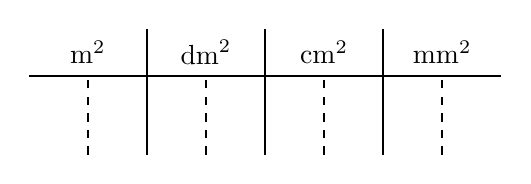
\begin{tikzpicture}
            \foreach \x in {0,1.5,3} \draw[thick] (\x,0) -- (\x,1.6);
            \foreach \x in {-0.75,0.75,2.25,3.75} \draw[thick, dashed] (\x,0) -- (\x,1);
            \draw[thick] (-1.5,1) -- (4.5,1);
            \foreach \eh/\x in {m/-0.75, dm/0.75, cm/2.25, mm/3.75} \node at (\x,1.3) {$\mathrm{\eh}^{2}$};
        \end{tikzpicture}
        \hspace{1cm}
        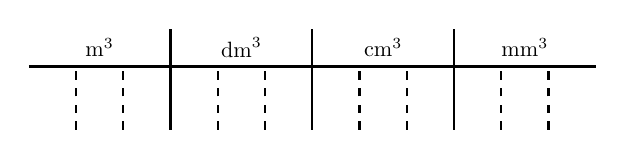
\begin{tikzpicture}[scale=0.8, transform shape]
            \foreach \x in {2.25,4.5,6.75} \draw[thick] (\x,0) -- (\x,1.6);
            \foreach \x in {0.75,1.5,3,3.75,5.25,6,7.5,8.25} \draw[thick, dashed] (\x,0) -- (\x,1);
            \draw[thick] (0,1) -- (9,1);
            \foreach \eh/\x in {m/1.125, dm/3.375, cm/5.625, mm/7.875} \node at (\x,1.3) {$\mathrm{\eh}^{3}$};
        \end{tikzpicture}
    \end{center}
\end{remark}

\begin{question}
    Hoeveel vierkante centimeter is $1 \, \mathrm{m}^{2}$?

    \begin{multipleChoice}
        \choice{$10^{2} \, \mathrm{cm}^{2}$}
        \choice{$10^{3} \, \mathrm{cm}^{2}$}
        \choice[correct]{$10^{4} \, \mathrm{cm}^{2}$}
        \choice{$10^{6} \, \mathrm{cm}^{2}$}
    \end{multipleChoice}

    \begin{solution}\nl
        $1 \, \mathrm{m} = 10^{2} \, \mathrm{cm}$, dus $1 \, \mathrm{m}^{2} = (10^{2} \, \mathrm{cm})^{2} = 10^{4} \, \mathrm{cm}^{2}$. Een vierkant van $1 \, \mathrm{m}$ op $1 \, \mathrm{m}$ bevat $100 \cdot 100$ vierkantjes van $1 \, \mathrm{cm}^{2}$.
    \end{solution}
\end{question}

\section{Samengestelde eenheden}\label{sec:samengestelde_eenheden}
Veel grootheden hebben een eenheid die een breuk is, zoals snelheid ($\mathrm{m/s}$) of massadichtheid ($\mathrm{kg/m^3}$). Je rekent met eenheden zoals met letters in de wiskunde.

\begin{proposition}[title={Omzetten van samengestelde eenheden}]\nl
    Zet de teller en de noemer \textbf{afzonderlijk} om en reken daarna de breuk uit. Een handige gevolgtrekking: $1 \, \mathrm{m/s} = 3{,}6 \, \mathrm{km/h}$.
\end{proposition}

\begin{example}[foldable=true,title={Voorbeeld: kilometer per uur naar meter per seconde}]\nl
    Een auto rijdt $50{,}0 \, \mathrm{km/h}$. Hoeveel meter per seconde is dit?

    \begin{solution}\nl
        \begin{align*}
            50{,}0 \, \mathrm{km/h} &= \frac{50{,}0 \cdot 10^{3} \, \mathrm{m}}{3600 \, \mathrm{s}} && \text{(teller: $1 \, \mathrm{km} = 10^{3} \, \mathrm{m}$, noemer: $1 \, \mathrm{h} = 3600 \, \mathrm{s}$)}\\
            &= 13{,}89 \, \mathrm{m/s} \simeq \boxed{1{,}39 \cdot 10^{1} \, \mathrm{m/s}} && \text{(uitrekenen)}
        \end{align*}
        Controle: $50{,}0 / 3{,}6 = 13{,}9$.
    \end{solution}
\end{example}

\begin{example}[foldable=true,title={Voorbeeld: kilogram per kubieke meter naar gram per kubieke centimeter}]\nl
    Een gas heeft een massadichtheid van $3{,}0 \, \mathrm{kg/m}^{3}$. Hoeveel gram per kubieke centimeter is dit?

    \begin{solution}\nl
        \begin{align*}
            3{,}0 \, \mathrm{kg/m}^{3} &= \frac{3{,}0 \cdot 10^{3} \, \mathrm{g}}{(10^{2} \, \mathrm{cm})^{3}} && \text{(teller: $1 \, \mathrm{kg} = 10^{3} \, \mathrm{g}$, noemer: $1 \, \mathrm{m} = 10^{2} \, \mathrm{cm}$)}\\
            &= \frac{3{,}0 \cdot 10^{3} \, \mathrm{g}}{10^{6} \, \mathrm{cm}^{3}} = \boxed{3{,}0 \cdot 10^{-3} \, \mathrm{g/cm}^{3}} && \text{(uitrekenen)}
        \end{align*}
    \end{solution}
\end{example}

\begin{question}
    Een fietser rijdt $36 \, \mathrm{km/h}$. Hoeveel is dat in meter per seconde?

    \begin{multipleChoice}
        \choice{$3{,}6 \, \mathrm{m/s}$}
        \choice[correct]{$10 \, \mathrm{m/s}$}
        \choice{$36 \, \mathrm{m/s}$}
        \choice{$130 \, \mathrm{m/s}$}
    \end{multipleChoice}

    \begin{solution}\nl
        $36 \, \mathrm{km/h} = \dfrac{36 \cdot 10^{3} \, \mathrm{m}}{3600 \, \mathrm{s}} = 10 \, \mathrm{m/s}$. Je deelt dus door $3{,}6$.
    \end{solution}
\end{question}

\section{Tijd}\label{sec:tijd_omzetten}
Bij tijd werk je niet met machten van 10: een uur telt 60 minuten en een minuut 60 seconden.

\begin{proposition}[title={Omzetten van tijd}]\nl
    \[ 1 \, \mathrm{min} = 60 \, \mathrm{s} \qquad 1 \, \mathrm{h} = 60 \, \mathrm{min} = 3600 \, \mathrm{s} \qquad 1 \text{ dag} = 24 \, \mathrm{h} = 86\,400 \, \mathrm{s} \]
    Het decimale deel van een uur is \textbf{geen} aantal minuten: $1{,}5 \, \mathrm{h}$ is $1 \, \mathrm{h}$ en $30 \, \mathrm{min}$, niet $1 \, \mathrm{h}$ en $50 \, \mathrm{min}$.
\end{proposition}

\begin{example}[foldable=true,title={Voorbeeld: decimale uren naar uren, minuten en seconden}]\nl
    Een rit duurt $8{,}43 \, \mathrm{h}$. Hoeveel uren, minuten en seconden is dit?

    \begin{solution}\nl
        Het gehele deel geeft $8 \, \mathrm{h}$. Het decimale deel zet je om naar minuten, en het decimale deel van de minuten naar seconden:
        \begin{align*}
            0{,}43 \, \mathrm{h} &= 0{,}43 \cdot 60 \, \mathrm{min} = 25{,}8 \, \mathrm{min} && \text{(dus $25 \, \mathrm{min}$ en een rest)}\\
            0{,}8 \, \mathrm{min} &= 0{,}8 \cdot 60 \, \mathrm{s} = 48 \, \mathrm{s} && \text{(rest naar seconden)}
        \end{align*}
        De rit duurt dus $\boxed{8 \, \mathrm{h} \; 25 \, \mathrm{min} \; 48 \, \mathrm{s}}$.
    \end{solution}
\end{example}

\begin{example}[foldable=true,title={Voorbeeld: minuten en seconden naar uur}]\nl
    Een proef duurt $3$ minuten en $13$ seconden. Hoeveel uur is dit?

    \begin{solution}\nl
        Deel het aantal minuten door 60 en het aantal seconden door 3600:
        \begin{align*}
            t &= \frac{3}{60} \, \mathrm{h} + \frac{13}{3600} \, \mathrm{h} && \text{($1 \, \mathrm{h} = 60 \, \mathrm{min} = 3600 \, \mathrm{s}$)}\\
            &= 0{,}0500 \, \mathrm{h} + 0{,}0036 \, \mathrm{h} = 0{,}0536 \, \mathrm{h} \simeq \boxed{5{,}36 \cdot 10^{-2} \, \mathrm{h}} && \text{(uitrekenen)}
        \end{align*}
    \end{solution}
\end{example}

\begin{question}
    Hoeveel is $2{,}25 \, \mathrm{h}$?

    \begin{multipleChoice}
        \choice{$2 \, \mathrm{h}$ en $25 \, \mathrm{min}$}
        \choice[correct]{$2 \, \mathrm{h}$ en $15 \, \mathrm{min}$}
        \choice{$2 \, \mathrm{h}$ en $2{,}5 \, \mathrm{min}$}
    \end{multipleChoice}

    \begin{solution}\nl
        $0{,}25 \, \mathrm{h} = 0{,}25 \cdot 60 \, \mathrm{min} = 15 \, \mathrm{min}$. Het decimale deel van een uur is geen aantal minuten.
    \end{solution}
\end{question}

\end{document}
